%(BEGIN_QUESTION)
% Copyright 2010, Tony R. Kuphaldt, released under the Creative Commons Attribution License (v 1.0)
% This means you may do almost anything with this work of mine, so long as you give me proper credit

Anta at voltmeteret i denne brokretsen viser en tydelig {\it negativ} spenning:

$$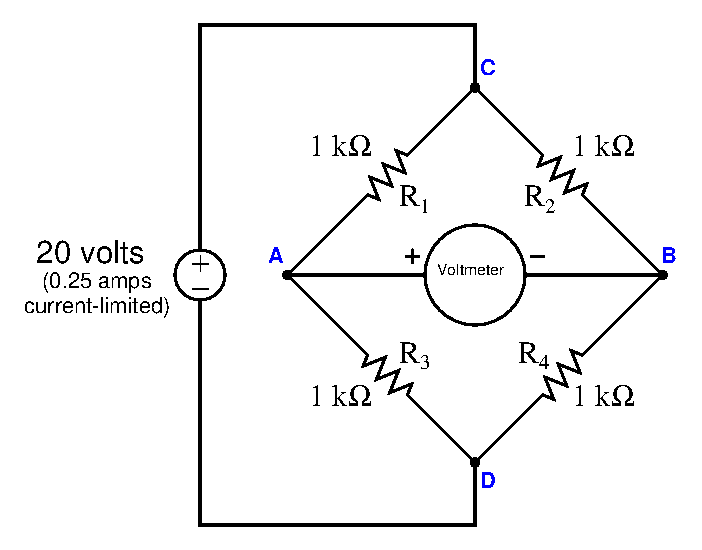
\includegraphics[width=15.5cm]{i00117x01.eps}$$

Vurder sannsynligheten for hver oppgitt feil i kretsen. Vurder én feil av gangen (ingen samtidige feil), og avgjør om feilen alene kan forklare {\it alle} målinger og symptomer i kretsen.

% No blank lines allowed between lines of an \halign structure!
% I use comments (%) instead, so that TeX doesn't choke.

$$\vbox{\offinterlineskip
\halign{\strut
\vrule \quad\hfil # \ \hfil & 
\vrule \quad\hfil # \ \hfil & 
\vrule \quad\hfil # \ \hfil \vrule \cr
\noalign{\hrule}
%
% First row
{\bf Feil} & {\bf Mulig} & {\bf Umulig} \cr
%
\noalign{\hrule}
%
% Another row
$R_1$ avbrudd &  &  \cr
%
\noalign{\hrule}
%
% Another row
$R_2$ avbrudd &  &  \cr
%
\noalign{\hrule}
%
% Another row
$R_3$ avbrudd &  &  \cr
%
\noalign{\hrule}
%
% Another row
$R_4$ avbrudd &  &  \cr
%
\noalign{\hrule}
%
% Another row
$R_1$ kortsluttet &  &  \cr
%
\noalign{\hrule}
%
% Another row
$R_2$ kortsluttet &  &  \cr
%
\noalign{\hrule}
%
% Another row
$R_3$ kortsluttet &  &  \cr
%
\noalign{\hrule}
%
% Another row
$R_4$ kortsluttet &  &  \cr
%
\noalign{\hrule}
%
% Another row
Spenningskilde død &  &  \cr
%
\noalign{\hrule}
} % End of \halign 
}$$ % End of \vbox

Angi til slutt hvilken {\it neste} diagnostiske test eller måling du ville gjort på systemet. Forklar hvordan resultatet av testen hjelper med å finne feilsted og/eller feiltype.

\vfil 

\underbar{file i00117}
\eject
%(END_QUESTION)





%(BEGIN_ANSWER)

% No blank lines allowed between lines of an \halign structure!
% I use comments (%) instead, so that TeX doesn't choke.

$$\vbox{\offinterlineskip
\halign{\strut
\vrule \quad\hfil # \ \hfil & 
\vrule \quad\hfil # \ \hfil & 
\vrule \quad\hfil # \ \hfil \vrule \cr
\noalign{\hrule}
%
% First row
{\bf Feil} & {\bf Mulig} & {\bf Umulig} \cr
%
\noalign{\hrule}
%
% Another row
$R_1$ avbrudd & $\surd$ &  \cr
%
\noalign{\hrule}
%
% Another row
$R_2$ avbrudd &  & $\surd$ \cr
%
\noalign{\hrule}
%
% Another row
$R_3$ avbrudd &  & $\surd$ \cr
%
\noalign{\hrule}
%
% Another row
$R_4$ avbrudd & $\surd$ &  \cr
%
\noalign{\hrule}
%
% Another row
$R_1$ kortsluttet &  & $\surd$ \cr
%
\noalign{\hrule}
%
% Another row
$R_2$ kortsluttet & $\surd$ &  \cr
%
\noalign{\hrule}
%
% Another row
$R_3$ kortsluttet & $\surd$ &  \cr
%
\noalign{\hrule}
%
% Another row
$R_4$ kortsluttet &  & $\surd$ \cr
%
\noalign{\hrule}
%
% Another row
Spenningskilde død &  & $\surd$ \cr
%
\noalign{\hrule}
} % End of \halign 
}$$ % End of \vbox


%(END_ANSWER)





%(BEGIN_NOTES)


%INDEX% Troubleshooting review: electric circuits (Wheatstone bridge)

%(END_NOTES)
